\documentclass[aspectratio=169]{beamer}
%\documentclass[aspectratio=169,handout]{beamer}
\usepackage[utf8]{inputenx} % For æ, ø, å
\usepackage{csquotes}       % Quotation marks
\usepackage{microtype}      % Improved typography
\usepackage{amssymb}        % Mathematical symbols
\usepackage{mathtools}      % Mathematical symbols
\usepackage[absolute, overlay]{textpos} % Arbitrary placement
\setlength{\TPHorizModule}{\paperwidth} % Textpos units
\setlength{\TPVertModule}{\paperheight} % Textpos units
\usepackage{tikz}
\usetikzlibrary{overlay-beamer-styles}  % Overlay effects for TikZ


\AtBeginSection{\frame{\sectionpage}}
\AtBeginSubsection{\frame{\subsectionpage}}

\usepackage{hyperref}
\usepackage{svg}
%\usefonttheme{serif}

\usepackage{xfrac}
\usepackage{soul} % Colored text and highlighting, respectively
\usepackage{xcolor}
\usepackage{tikz-cd} % For commutative diagrams
\usepackage{tikz-3dplot}
\usetikzlibrary{angles}
\RequirePackage{pgfplots}
\usepackage{mathtools}
\usepackage{answers}
\usepackage{setspace}
\usepackage{graphicx}
\usepackage{enumerate}
\usepackage{multicol}
%\usepackage{mathrsfs}
\usepackage{amsmath,amsthm}
\usepackage{marvosym,wasysym} %fucking smileys
\usepackage{float}
\usepackage{morefloats}
\usepackage{pgf,tikz}
\pgfplotsset{compat=1.15}
%\usepackage{mathrsfs}
\usetikzlibrary{arrows}
\usepackage{subcaption}
\usepackage[most]{tcolorbox}
\tcbuselibrary{theorems}
\usepackage{fancyvrb}
\usepackage{longtable,booktabs}
\usepackage{stackrel}
\usepackage{animate}
\usepackage[percent]{overpic}
\definecolor{lighter_csu_green}{RGB}{60,133,77}
\definecolor{csu_gold}{RGB}{198,184,77}
\definecolor{gray}{RGB}{60,60,60}
\newcommand\boldgreen[1]{\textcolor{lighter_csu_green}{\emph{\textbf{#1}}}}
\newcommand\boldgold[1]{\textcolor{csu_gold}{\textbf{#1}}}
\usepackage{MnSymbol}
%border matrix
\makeatletter
\newif\if@borderstar
\def\bordermatrix{\@ifnextchar*{%
\@borderstartrue\@bordermatrix@i}{\@borderstarfalse\@bordermatrix@i*}%
}
\def\@bordermatrix@i*{\@ifnextchar[{\@bordermatrix@ii}{\@bordermatrix@ii[()]}}
\def\@bordermatrix@ii[#1]#2{%
\begingroup
\m@th\@tempdima8.75\p@\setbox\z@\vbox{%
\def\cr{\crcr\noalign{\kern 2\p@\global\let\cr\endline }}%
\ialign {$##$\hfil\kern 2\p@\kern\@tempdima & \thinspace %
\hfil $##$\hfil && \quad\hfil $##$\hfil\crcr\omit\strut %
\hfil\crcr\noalign{\kern -\baselineskip}#2\crcr\omit %
\strut\cr}}%
\setbox\tw@\vbox{\unvcopy\z@\global\setbox\@ne\lastbox}%
\setbox\tw@\hbox{\unhbox\@ne\unskip\global\setbox\@ne\lastbox}%
\setbox\tw@\hbox{%
$\kern\wd\@ne\kern -\@tempdima\left\@firstoftwo#1%
\if@borderstar\kern2pt\else\kern -\wd\@ne\fi%
\global\setbox\@ne\vbox{\box\@ne\if@borderstar\else\kern 2\p@\fi}%
\vcenter{\if@borderstar\else\kern -\ht\@ne\fi%
\unvbox\z@\kern-\if@borderstar2\fi\baselineskip}%
\if@borderstar\kern-2\@tempdima\kern2\p@\else\,\fi\right\@secondoftwo#1 $%
}\null \;\vbox{\kern\ht\@ne\box\tw@}%
\endgroup
}
\makeatother

\usetheme{UiB}

%For easier reading
\setbeamersize{text margin left=40pt,text margin right=40pt}
\renewcommand{\baselinestretch}{1.3}


%% FONT STUFF
\usefonttheme[onlymath]{serif}

%Commands
\newcommand{\R}{\mathbb{R}}
\newcommand{\C}{\mathbb{C}}
\newcommand{\opens}{\mathcal{O}}
\newcommand{\hilbert}{\mathcal{H}}
\newcommand{\algebra}{\mathcal{A}}
\newcommand{\ideals}{\mathcal{I}}
\newcommand{\functionals}{\mathcal{M}}
\newcommand{\spec}{\mathrm{spec}}
\newcommand{\clifford}{\mathrm{C}\ell}
    \newcommand\quotient[2]{
        \mathchoice
            {% \displaystyle
                \text{\raise1ex\hbox{$#1$}\Big/\lower1ex\hbox{$#2$}}%
            }
            {% \textstyle
                #1\,/\,#2
            }
            {% \scriptstyle
                #1\,/\,#2
            }
            {% \scriptscriptstyle  
                #1\,/\,#2
            }
    }

% Special Commands
\newcommand{\bigslant}[2]{{\raisebox{.2em}{$#1$}\left/\raisebox{-.2em}{$#2$}\right.}}
\newcommand{\RE}{\mathrm{Re}}
\newcommand{\IM}{\mathrm{Im}}
\newcommand{\multivectorbundle}{\mathcal{G}(M,g)}
\newcommand{\multivectorfields}{\mathcal{G}(M)}
\newcommand{\differentialforms}{\mathcal{G}^*(M)}
\newcommand{\kvectorfields}[1]{\mathcal{G}^{#1}(M)}
\newcommand{\evenfields}{\mathcal{G}^{[0]}(M)}
\newcommand{\oddfields}{\mathcal{G}^{[1]}(M)}
\newcommand{\id}{\mathrm{id}}
\newcommand{\innerproduct}[2]{\left\langle #1, #2 \right\rangle_{L_2(\Sigma)}}
%\newcommand{\algebra}[1]{\mathcal{A}_{#1}}
\newcommand{\grad}{\boldsymbol{\nabla}}
\newcommand{\dirac}{\boldsymbol{D}}
\newcommand{\geometricalg}{\mathcal{G}(V)}
\newcommand{\spacealg}{\mathcal{G}_3}
\newcommand{\dual}[1]{\overset{$\star$}&{#1}}
\newcommand{\G}{\mathcal{G}}
\newcommand{\cauchy}{\mathcal{C}}
\newcommand{\poisson}{\mathcal{P}}
\newcommand{\tangent}{\boldsymbol{t}}

\newcommand{\openO}{\mathcal{O}}
\newcommand{\openU}{\mathcal{U}}
\newcommand{\characters}{\mathfrak{M}}
\newcommand{\Span}{\operatorname{Span}}
\newcommand{\paravectors}{\mathcal{P}}
\newcommand{\paravectorfields}{\mathcal{P}(M)}
\newcommand{\monogenics}{\mathcal{M}}
\newcommand{\dualmonogenics}{\mathcal{M}^*}
\newcommand{\Grassmannian}[2]{\textrm{Gr}(#1,#2)}
\newcommand{\spinalgebra}{\mathfrak{spin}(n)}
\newcommand{\spingroup}{\operatorname{Spin}(n)}
\newcommand{\ball}{\mathbb{B}}
\newcommand{\disk}{\mathbb{D}}
\newcommand{\projection}{\operatorname{P}}
\newcommand{\vectorspace}{\mathbb{V}}
\newcommand{\multivectorfieldson}[1]{\mathcal{G}(#1)}
\newcommand{\biparavectorfieldson}[1]{\mathcal{G}_n(#1)^{0+2}}
\newcommand{\spinnorm}[1]{\|#1\|_{L_2}}
\newcommand{\rejection}{\operatorname{R}}
\newcommand{\vectorpotential}{\mathbf{A}}
\newcommand{\current}{\blade{j}}
\newcommand{\magneticbivector}{\blade{b}}
\newcommand{\cross}{\boldsymbol{\times}}
\newcommand{\blade}[1]{\boldsymbol{#1}}
\newcommand{\intcurrent}[1]{\left[ #1 \right]}
\newcommand{\multivecinnerproduct}[2]{\ll #1, #2\gg}
\newcommand{\spacetime}{\boldsymbol{\gamma}}
\newcommand{\gradst}{\boldsymbol{\nabla}_{\textrm{ST}}}
\newcommand{\boundary}{{\partial M}}
\newcommand{\normalcurrent}{\blade{j}^{\blade{\nu}}}
\newcommand{\tangentialcurrent}{\blade{j}^{\blade{I}_\partial}}
\newcommand{\normal}{\blade{\nu}}
\newcommand{\pseudoscalar}{\blade{I}}

\newcommand{\kforminnerproduct}[2]{\llangle #1, #2 \rrangle}

\DeclarePairedDelimiter\angles{\langle}{\rangle}
\newcommand{\proj}[2]{\angles*{#2}_{#1}}

% Forms stuff
\newcommand{\harmonicfields}[1]{\mathcal{H}^{#1}(M)}
\newcommand{\monogenicex}[1]{\mathcal{M}^{#1}_{\textrm{ex}}(M)}
\newcommand{\monogenicco}[1]{\mathcal{M}^{#1}_{\textrm{co}}(M)}
\newcommand{\monogenicdirichlet}[1]{\mathcal{M}^{#1}_D(M)}
\newcommand{\monogenicneumann}[1]{\mathcal{M}^{#1}_N(M)}
\newcommand{\exactfields}[1]{\mathcal{E}^{#1}(M)}
\newcommand{\coexactfields}[1]{\mathcal{C}^{#1}(M)}
\newcommand{\monogenicfields}[1]{\mathcal{M}^{#1}(M)}
\newcommand{\cliffordoplus}{\stackrel{C\ell}{\oplus}}
\newcommand{\bivector}{\blade{B}}

\author{Colin Roberts}
\setbeamercolor{title}{fg=white} 
\title{Clifford Analysis and a Noncommutative Gelfand Representation}
\setbeamercolor{subtitle}{fg=white} 
\subtitle{}

\setcounter{tocdepth}{1}

\begin{document}

\begin{frame}{Overview}
\tableofcontents
\end{frame}

\section{Introduction}

\begin{frame}{Motivating problems}
\vfill
\begin{itemize}
\pause
\item \boldgreen{Electrical Impedance Tomography (EIT)} asks whether one can determine the conductivity of a medium from the voltage-to-current map.
\pause
\item The \boldgreen{Calder\'on problem} replaces the medium with a manifold $M$, conductivity with $g$, and replaces the voltage-to-current map with the Dirichlet-to-Neumann operator $\Lambda$.
\end{itemize}
\vfill
\end{frame}

\begin{frame}{Other questions}
\vfill 
    \begin{itemize}
        \pause 
        \item What topological information can we retrieve from functions on a manifold $M$?

        \pause
        \item Do these functions also contain geometric information such as metric data?

        \pause
        \item How much can we learn about $M$ if our data is supported only on the boundary?
    \end{itemize}
\vfill
\end{frame}

\subsection{Preliminaries}

\begin{frame}{}
\vfill
\begin{itemize}
    \pause
    \item \boldgreen{Clifford algebra} originated in 1878 with William Kingdon Clifford's work that extends Hermann Grassmann's \boldgreen{exterior algebra}. 
    \pause
    \item \boldgreen{Clifford analysis} arrived in the 1980's due to Hestenes, Sobczyk, Sommen, Brackx, and Delenghe in order to enrich \'Elie Cartan's \boldgreen{differential forms}. See: \boldgold{[Hestenes, Sobczyk: 1984]} and \boldgold{[Doran, Lasenby: 2003]}.
\end{itemize}
\vfill
\end{frame}

\begin{frame}{Clifford algebras}
\vfill
\pause
Let $V$ be a vector space over a field $\mathbb{F}$ with quadratic form $Q$.
\begin{itemize}
        \pause
        \item Define the tensor algebra
        \[
        \mathcal{T}(V) \coloneqq \bigoplus_{j=0}^\infty V^{\otimes_j} = \mathbb{F} \oplus (V \otimes V) \oplus (V \otimes V \otimes V) \oplus \cdots.
        \]
        \pause
        \item Form the \boldgreen{Clifford algebra} via a quotient
        \[
        C\ell(V,Q) \coloneqq \mathcal{T}(V)/ \langle \blade{v} \otimes \blade{v} - Q(\blade{v})\rangle.
        \]
\end{itemize}
\vfill
\end{frame}

\begin{frame}{Geometric and exterior algebras}
\vfill
\begin{itemize}
        \pause
        \item Given a (pseudo) inner product $g$, we set $Q(\cdot)=g(\cdot,\cdot)$ and define a \boldgreen{geometric algebra}
        \[
        \G \coloneqq C\ell(V,g).
        \]
        \pause
        \item The \boldgreen{exterior algebra} is given by
        \[
        \bigwedge(V) \coloneqq C\ell(V,0).
        \]
\end{itemize}
\vfill
\end{frame}

\begin{frame}{Algebraic structure}
\vfill
\pause
Multiplication in $\G$ is seen by looking at how $\otimes$ acts in the quotient.
\begin{itemize}
    \pause
    \item Given $\blade{u}, \blade{v} \in \G$ we can take the product
    \[
    \blade{u}\blade{v} = \underbrace{\blade{u}\cdot \blade{v}}_{\textrm{scalar}} + \underbrace{\blade{u}\wedge \blade{v}}_{\textrm{bivector}}.
    \]
\begin{itemize}
    \pause
    \item The scalar part is symmetric: $\blade{u}\cdot \blade{v} = g(\blade{u},\blade{v})$.
    \pause
    \item The bivector part is antisymmetric: $\blade{u}\wedge \blade{v} = -\blade{v}\wedge \blade{u}$.
\end{itemize}
\end{itemize}
\vfill
\end{frame}

\begin{frame}{Multivectors}
\vfill
\begin{itemize}
    \pause
        \item $\G$ is graded and of dimension $2^n$.
    \begin{itemize}
        \pause
        \item There are ${n \choose r}$ elements in the space of grade-$r$ elements, $\G^r$, called \boldgreen{$r$-vectors}. 
        \pause
        \item Those that are exterior products of $r$ independent vectors are \boldgreen{$r$-blades}. E.g., $\blade{A_r}=\blade{v}_1 \wedge \cdots \wedge\blade{v}_r$.
        \pause
        \item Elements of the even grade subalgebra, $\G^+$, are called \boldgreen{spinors}.
    \end{itemize}
        \pause
        \item The most general elements are \boldgreen{multivectors} and are given by
        \[
        A = \sum_{r=0}^n \proj{r}{A},
        \]
        where $\proj{r}{A}\in \G^r$ extracts the grade $r$ part of $A$. So $\displaystyle{\G=\bigoplus_{r=0}^n \G^r}$.
\end{itemize}
\vfill
\end{frame}

\begin{frame}{Algebraic Structure}
\vfill
\begin{itemize}
\pause
\item Extend the multiplication from vectors to multivectors. 
\pause
\item On homogeneous elements,
\[
A_r B_s = \proj{|r-s|}{A_r B_s} + \proj{|r-s|+2}{A_r B_s} + \cdots + \proj{r+s}{A_r B_s}
\]
\pause
\item The most important products are
\begin{align*}
A_r \cdot B_s &\coloneqq \proj{|r-s|}{A_r B_s}  & A_r \wedge B_s &\coloneqq \proj{r+s}{A_r B_s}\\
~\\
A_r \rfloor B_s &\coloneqq \proj{s-r}{A_r B_s}  & A_r \lfloor B_s &\coloneqq \proj{r-s}{A_r B_s}
\end{align*}
\end{itemize}
\vfill
\end{frame}

\begin{frame}{Reciprocals and reverses}
\vfill
\begin{itemize}
\pause
\item Given any vector basis $\blade{v}_i$, define the \boldgreen{reciprocal vectors} by $\blade{v}^i\cdot \blade{v}_j = \delta^i_j$.
\pause
\item The \boldgreen{reverse} of a multivector is extended linearly from the action on $r$-blades by
\[
\blade{A_r}^\dagger = (\blade{v}_1 \wedge \cdots \wedge\blade{v}_r)^\dagger = \blade{v}_r \wedge \cdots \wedge\blade{v}_1.
\]
\end{itemize}
\vfill
\end{frame}


\begin{frame}{Inner product and norm}
\vfill
\begin{itemize}
\pause
\item Define the \boldgreen{multivector inner product} by
\[
(A,B) \coloneqq \proj{}{A^\dagger B}
\]
which is bilinear, symmetric, and positive definite if $g$ is positive definite. 
\pause
\item Define the \boldgreen{multivector norm} by
\[
|A| \coloneqq \sqrt{(A,A)}.
\]
\end{itemize}
\vfill
\end{frame}

\begin{frame}{Adjoint}
\vfill
Note the reverse acts as an adjoint by
\begin{align*}
(CA,B) &= (A,C^\dagger B)\\
(AC,B) &= (A,BC^\dagger).
\end{align*}
\vfill
\end{frame}

\begin{frame}{Pseudoscalars}
\vfill
\begin{itemize}
\pause
\item \boldgreen{Pseudoscalars} are the grade-$n$ elements. For example, the volume element 
\[
\blade{\mu} = \blade{v}_1 \wedge \cdots \wedge \blade{v}_n.
\]
\pause  
\item We define the \boldgreen{unit pseudoscalar} by 
\[
\pseudoscalar \coloneqq \frac{1}{|\blade{\mu}|} \blade{\mu}.
\]
\end{itemize}
\vfill
\end{frame}

\begin{frame}{Blades and subspaces}
\vfill
\begin{itemize}
\pause
\item If $g$ is positive definite all blades are invertible \boldgold{[Chisholm: 2012]}.
\pause
\item If $|\blade{A_r}|=1$, then $\blade{A_r}$ is a \boldgreen{unit blade}. 
\pause
\item Unit $r$-blades correspond to $r$-dimensional subspaces so they correspond to points in $\Grassmannian{r}{n}$.
\end{itemize}
\vfill
\end{frame}

\begin{frame}{Duality}
\vfill
\begin{itemize}
\pause
\item Given any multivector $A$, we can take its \boldgreen{dual}
\[
A^\perp \coloneqq A \pseudoscalar^{-1}.
\]
\pause
\item Note $A_r^\perp \in \G^{n-r}$, like the Hodge star $\star$.
\end{itemize}
\vfill
\end{frame}

\begin{frame}{Projection and rejection}
\vfill
\begin{itemize}
\pause
\item The \boldgreen{projection} of $B$ into a subspace $\blade{A_r}$ by
\[
\projection_{\blade{A_r}} (B) \coloneqq B\rfloor \blade{A_r}\blade{A_r}^{-1}
\]
\pause
\item The \boldgreen{rejection} by
\[
\rejection_{\blade{A_r}} (B) \coloneqq B\wedge \blade{A_r}\blade{A_r}^{-1}.
\]
\pause
\item Both are grade preserving.
\end{itemize}
\vfill
\end{frame}

\begin{frame}{Examples}
\vfill
\begin{itemize}
\pause
\item Define $\G_{p,q}$ by letting $\blade{e}_i^2=-1$ for $i=1,\dots,p$ and $\blade{e}_i^2=+1$ otherwise.
\pause
\item \underline{\textbf{Claim:}} $\mathbb{H}$ arises naturally as the even subalgebra $\G_3^+\coloneqq \G_{0,3}^+$.

\pause
\item \underline{\textbf{Claim:}} $\C$ arises naturally as the even subalgebra $\G_2^+\coloneqq \G_{0,2}^+$.
\begin{itemize}
\pause
\item Take the standard basis $\blade{e}_1,\blade{e}_2$, and define $\bivector_{12}= \blade{e}_1\blade{e}_2$ and note $\bivector_{12}^2 = -1$. Thus,
\[
(u_1+v_1 \bivector_{12})(u_2 + v_2 \bivector_{12}) = u_1u_2-v_1 v_2 + (u_1 v_2+u_2v_1)\bivector_{12}.
\]
\pause
\item Right multiplication by $\bivector_{12}$ rotates counter-clockwise by $\pi/2$.
\end{itemize}
\end{itemize}
\vfill
\end{frame}

\section{Clifford analysis}

\begin{frame}{Multivector Fields}
\vfill
\begin{itemize}
\pause
\item Let $M$ be a smooth, compact, connected, and oriented $n$-dimensional Riemannian manifold with metric $g$.
\pause
\item \noindent\textbf{\underline{Idea:}} Form the Clifford algebras on tangent spaces.
    \begin{itemize}
        \pause
        \item Each $C\ell(T_pM,g_p)$ is a \boldgreen{geometric tangent space} which we glue together to form
        \[
        C\ell(TM,g) \coloneqq \bigsqcup_{p\in M} C\ell(T_pM,g_p).
        \]
        \pause
        \item The space of \boldgreen{(smooth) multivector fields} is
        \[
        \G(M) \coloneqq \{\textrm{$C^\infty$-smooth sections of $C\ell(TM,g)$}\}.
        \]
    \end{itemize}
    \pause
    \item Retain the same naming scheme as before.
\end{itemize}
\vfill
\end{frame}

\begin{frame}{Multivector derivative}
\vfill
\pause
    On $M$, take the unique Levi-Civita connection $\nabla$ and covariant derivative $\nabla_{\blade{u}}$.
    \pause
    \begin{itemize}
        \item $\nabla_{\blade{u}}$ is extended to multivectors and is grade preserving \boldgold{[Schindler: 2018]},
        \[
        \nabla_{\blade{u}} A_r = \proj{r}{\nabla_{\blade{u}} A_r}.
        \]
        \pause
        \item $\nabla_{\blade{u}}$ is compatible with dot and wedge since
        \begin{align*}
        \nabla_{\blade{u}}(A\cdot B) &= (\nabla_{\blade{u}} A)\cdot B + A \cdot (\nabla_{\blade{u}} B)\\
        \nabla_{\blade{u}}(A\wedge B) &= (\nabla_{\blade{u}} A) \wedge B + A \wedge (\nabla_{\blade{u}} B).
        \end{align*}
    \end{itemize}
\vfill
\end{frame}

\begin{frame}{Gradient}
\vfill
\begin{itemize}
    \pause
    \item Define the \boldgreen{gradient} (or \boldgreen{Dirac operator}) locally by
    \[
    \grad = \sum_{i=1}^n \blade{v}^i \nabla_{\blade{v}_i}
    \]
    \pause
    \item $\grad$ acts as a vector in $\G(M)$ and obeys the Leibniz rule
    \[
    \grad(AB) = \dot{\grad}\dot{A}B + \dot{\grad}A\dot{B}.
    \]
    \pause
    \item Note $\grad^2=\Delta$, the Laplace-Beltrami operator.
\end{itemize}
\vfill
\end{frame}

\begin{frame}{Example}
\vfill
\begin{itemize}
\pause
\item In $\G_3(\R^3)$, $\nabla_{\blade{e}_i}$ is the partial derivative.
\pause
\item Take a vector field $\blade{v}$, then
    \[
    \grad \blade{v} = \underbrace{\grad \cdot \blade{v}}_{\textrm{divergence}} + \underbrace{\grad \wedge \blade{v}}_{\textrm{curl}}.
    \]
\pause
\item Specifically,
\[
    \operatorname{curl}(\blade{v}) = (\grad \wedge \blade{v})^\perp
\]
\end{itemize}
\vfill
\end{frame}

\begin{frame}{Differential forms}
\vfill
\begin{itemize}
    \pause
    \item Define the \boldgreen{$r$-dimensional directed measure}
    \[
    dX_r\coloneqq \blade{v}_{j_1} \wedge \cdots \wedge \blade{v}_{j_r} dx^{j_1} \cdots dx^{j_r}
    \] 
    where $1\leq j_1<\cdots<j_r\leq n$ and summation is implied. 
    \pause
    \item Define an $r$-form $a_r$ by
    \[
    \alpha_r = A_r \cdot dX_r^\dagger
    \]
    where $A_r = \frac{1}{r!} a_{i_1 \cdots i_r} \blade{v}^{i_1} \wedge \cdots \wedge \blade{v}^{i_r}$. 
    \pause
    \item Refer to $A_r$ the \boldgreen{multivector equivalent} of $\alpha_r$.
\end{itemize}
\vfill
\end{frame}

\begin{frame}{Exterior algebra and calculus}
\vfill
\begin{itemize}
\pause
\item Given $r$-forms $a_r$, $b_r$, and an $s$-form $c_s$, we have
\begin{align*}
a_r + b_r &= (A_r+B_r) \cdot dX_r^\dagger, & a_r \wedge c_s &= (A_r \wedge C_s) \cdot dX_{r+s}^\dagger.
\end{align*}
\vspace*{-0.25cm}
\pause
\item The exterior derivative on multivector equivalents is 
\[
da_r = (\grad \wedge A_r) \cdot dX_{r+1}^\dagger
\]
\pause
\vspace*{-0.25cm}
\item The Hodge star on multivector equivalents is
\[
\star a_r = (\pseudoscalar^{-1} A_r)^\dagger \cdot dX_{n-r}^\dagger
\]
\end{itemize}
\vfill
\end{frame}

\begin{frame}{Volume form}
\vfill
\begin{itemize}
    \pause
    \item The \boldgreen{volume form} on $M$ is given in local coordinates by 
    \[
    \mu = \sqrt{|g|}dx^1\cdots dx^n = \pseudoscalar^{-1} \cdot dX_n
    \]
    \pause
    \item We integrate scalar fields $A_0$ on $M$ by
    \[
    \int_M A_0^\perp \cdot dX_n =  \int_M A_0 \mu.
    \]
\end{itemize}
\vfill
\end{frame}

\begin{frame}{Multivector field inner product}
\vfill
\begin{itemize}
\pause
\item We define the $L^2$-inner product on multivector fields by 
\[
\multivecinnerproduct{A}{B}~ \coloneqq \frac{1}{\textrm{vol}(M)} \int_M (A,B)\mu
\]
\vspace*{-0.1cm}
\pause
\item This realizes the $r$-form inner product
\[
\int_M \alpha_r \wedge \star \beta_r = \int_M \proj{}{A_r^\dagger B_r}\mu = \textrm{vol}(M)\multivecinnerproduct{A}{B}
\]
\vspace*{-0.1cm}
\pause
\item $\multivecinnerproduct{A_r}{B_s}=0$ when $r\neq s$ so the $L^2$-direct sum agrees with the grade based direct sum.
\end{itemize}
\vfill
\end{frame}

\begin{frame}{Boundary}
\vfill
\begin{itemize}
\pause
\item On $\partial M$, the boundary pseudoscalar $\pseudoscalar_{\partial}$ induces the boundary normal 
\[
\blade{\nu} = \pseudoscalar_\partial^\perp.
\]
\vspace*{-0.25cm}
\pause
\item The boundary volume form is
\[
\mu_\partial \coloneqq \pseudoscalar_\partial^{-1} \cdot dX_{n-1}
\] 
and we define 
\[
\multivecinnerproduct{A}{B}_\partial~ \coloneqq \frac{1}{\textrm{vol}(M)}\int_{\boundary} (A,B)\mu_\partial.
\]
\end{itemize}
\vfill
\end{frame}

\begin{frame}{Multivector valued integrals}
\vfill
We can define a multivector valued integral on an oriented submanifold $R$ by taking $A\in \G(M)$ and computing
\[
\int_R A \pseudoscalar_R \mu_R.
\]
\vfill
\end{frame}

\begin{frame}{}
\vfill
\begin{theorem}[Hestenes, Sobczyk, 1984]
Let $A,B \in \G(M)$, then
\begin{align*}
\int_M \dot{A}\dot{\grad}\pseudoscalar \mu &= \int_\boundary A \pseudoscalar_\partial \mu_\partial\\
\int_M \pseudoscalar \grad B \mu &= \int_\boundary \pseudoscalar_\partial B\mu_\partial\\
\int_M \dot{A}\dot{\grad} \pseudoscalar B \mu &= (-1)^n \int_M A \pseudoscalar \grad B \mu + \int_\boundary A \pseudoscalar_\partial B \mu_\partial.
\end{align*}
\end{theorem}
\vfill
\end{frame}

\begin{frame}{}
\vfill
\begin{theorem}
We have the Green's formula for the gradient
\[
\multivecinnerproduct{A}{\pseudoscalar \grad B} = (-1)^n \multivecinnerproduct{\grad A}{\pseudoscalar B} + \multivecinnerproduct{A}{\pseudoscalar_\partial B}_\partial.
\]
\end{theorem}
%
%\emph{Proof.} Fix $A^\dagger,B \in \G(M)$ and note that
%\begin{align*}
%    \int_M A^\dagger \pseudoscalar \grad B \mu &= (-1)^n \int_M \dot{A}^\dagger \dot{\grad} \pseudoscalar B \mu + \int_{\partial M} A^\dagger \pseudoscalar_\partial B \mu_\partial\\
%    &=(-1)^n \int_M (\grad A)^\dagger \pseudoscalar B \mu + \int_{\partial M} A^\dagger \pseudoscalar_\partial B \mu_\partial.
%\end{align*}
%Take the scalar part and divide by $\textrm{vol}(M)$ to find
%\[
%\multivecinnerproduct{A}{\pseudoscalar \grad B} = (-1)^n \multivecinnerproduct{\grad A}{\pseudoscalar B} + \multivecinnerproduct{A}{\pseudoscalar_\partial B}_\partial.
%\]
\vfill
\end{frame}


\begin{frame}{Special fields}
\vfill
\begin{itemize}
\pause
\item Define the \boldgreen{monogenic fields}
\[
\monogenicfields{} ~\coloneqq \{ A \in \G(M) ~\vert~ \grad A = 0 \}.
\]
\vspace*{-0.25cm}
\pause
\item Let $f=u+v\blade{B} \in \G_2^+(\R^2)$ then $\grad f = 0$ yields the Cauchy-Riemann equations
\begin{align*}
    \frac{\partial u}{\partial x} &= \frac{\partial v}{\partial y}, &
    \frac{\partial u}{\partial y} &= -\frac{\partial v}{\partial x}.
\end{align*}
\pause
\vspace*{-0.25cm}
\item Define the \boldgreen{gradients}
\[
\grad \G(M) \coloneqq \{\grad A ~\vert~ A \in \G(M) \textrm{~and~} A\vert_\boundary = 0 \}.
\]
\end{itemize}
\vfill
\end{frame}

\begin{frame}{Cauchy kernel}
\vfill
\begin{itemize}
\pause
\item For the remainder, take $M$ imbedded in $\R^n$ with $n\geq 2$.
\pause
\item Define the vector field
\[
E(x) \coloneqq \frac{1}{S_n} \frac{x}{|x|^n}
\]
where $S_n$ is the surface area of the unit ball. 
\pause
\item Note,
\[
\grad E(x) = -\dot{E}(x)\dot{\grad} = \delta(x).
\]
\pause
\item Define the \boldgreen{Cauchy kernel} by $G(x,x')\coloneqq E(x'-x)$.
\end{itemize}
\vfill
\end{frame}

\begin{frame}{Cauchy integral}
\vfill
\begin{itemize}
\pause
\item Let $A\in \monogenicfields{}$, then we have the \boldgreen{Cauchy integral formula}
\[
A(x) = (-1)^n \pseudoscalar^{-1} \int_\boundary G(x,x') \pseudoscalar_\partial(x') A(x') \mu_\partial(x').
\]
\pause
\item This uniquely determines a monogenic field from boundary values.
\end{itemize}
\vfill
\end{frame}

\begin{frame}{}
\vfill
\begin{lemma}
Let $A\in \monogenicfields{}$ be such that $A\vert_\boundary = 0$. Then $A=0$ on all of $M$.
\end{lemma}
\begin{lemma}
Fix a multivector field $A\in \G(M)$. If
\[
\multivecinnerproduct{A}{B}=0
\]
for all $B\in \G(M)$ with $B\vert_{\boundary} = 0$, then $A=0$.
\end{lemma}
\vfill
\end{frame}

%\begin{frame}{Proof}
%We note
%\[
%|A| \leq |\pseudoscalar^{-1}| \left| \int_\boundary G(x,x')\pseudoscalar_\partial(x') A(x')\mu_\partial(x')\right| \leq \int_\boundary\left|  G(x,x')\pseudoscalar_\partial(x') A(x') \right|\mu_\partial(x') = 0
%\]
%thus $A=0$ on $M$.
%\end{frame}

%\begin{frame}{}
%\vfill
%\emph{Proof sketch.}
%\begin{itemize}
%\pause
%\item Use mollifiers to smooth indicator functions $\chi_U$ on open subsets $U$ to be supported only on closed $\epsilon$ neighborhood $\overline{U^\epsilon}$. Call these functions $\chi_U^\epsilon$.
%\pause
%\item Write $A=\sum_J A_J \blade{V}^J$ with $\blade{V}^J = \blade{v}^{j_1}\wedge \cdots\wedge  \blade{v}^{j_r}$. Then note
%    \[
%    \multivecinnerproduct{A}{A_J \blade{V}_J \chi_U^\epsilon} = 0
%    \] 
%    implies $A_J=0$ on $U^\epsilon$ for all $J$ since $(\blade{V}^{J}, \blade{V}_K)=\delta^J_K$. Hence $A=0$ on $U^\epsilon$.
%\pause
%\item Cover $M$ in such $U^\epsilon$ and repeat the argument leaving the $A\vert_\boundary$ undetermined. But, by smoothness of $A$, $A=0$ on $\partial M$.
%\end{itemize}
%\vfill
%\end{frame}

\begin{frame}{}
\vfill
\begin{theorem}[Clifford-Hodge-Morrey Decomposition]
The space of multivector fields $\G(M)$ has the $L^2$-orthogonal decomposition
\[
\G(M) = \monogenicfields{} \oplus \pseudoscalar \grad \G(M).
\]
\end{theorem}
\vfill
\end{frame}

\begin{frame}
\vfill
\emph{Proof.}
\begin{itemize}
\pause
\item \emph{Orthogonality:} Let $A \in \monogenicfields{}$ and $\pseudoscalar \grad B \in \pseudoscalar \grad \G(M)$ and note
\[
\multivecinnerproduct{A}{\pseudoscalar \grad B} = (-1)^n \multivecinnerproduct{\grad A}{\pseudoscalar B} + \multivecinnerproduct{A}{\pseudoscalar_\partial B} = 0,
\]
by the multivector Green's formula.
\end{itemize}
\vfill
\end{frame}

\begin{frame}{}
\vfill
\begin{itemize}
\pause
\item Let $C\in \G(M)$ be in the orthogonal complement to $\pseudoscalar \grad \G(M)$. 
\pause
\item Use the Cauchy integral formula, construct a monogenic field $\tilde{C}$ from $C\vert_\boundary$ and note $C=\tilde{C}+C_0$ where $C_0\vert_\boundary = 0$. 
\pause
\item Note,
\[
0 = \multivecinnerproduct{C}{\pseudoscalar \grad B} = \multivecinnerproduct{\grad C_0}{\pseudoscalar B}.
\]
\pause
\item By the previous lemmas, it must be that $C_0=0$. Hence the orthogonal complement to $\pseudoscalar \grad \G(M)$ is $\monogenicfields{}$.
\end{itemize}
\vfill
\end{frame}

\begin{frame}{Comparing to Hodge-Morrey}
\vfill
\begin{itemize}
\pause
\item The Hodge-Morrey decomposition reads
\[
\Omega^r(M) = \underbrace{\mathcal{E}_D^r(M)}_{\operatorname{Im}(\grad \wedge)} \oplus \underbrace{\mathcal{C}_N^r(M)}_{\operatorname{Im}(\grad \rfloor)} \oplus \underbrace{\mathcal{H}^r(M)}_{\operatorname{Ker}(\grad)}.
\]
via \boldgold{[Schwarz: 1995]}.
\pause 
\item Whereas the Clifford-Hodge-Morrey decomposition ignores specific grades
\[
\G(M) = \monogenicfields{} \oplus \pseudoscalar \grad \G(M).
\]
\end{itemize}
\vfill
\end{frame}

\section{Gelfand theory}

\begin{frame}{Open questions}
\vfill
\begin{itemize}
\pause
    \item In \boldgold{[Belishev: 2003]}, we see an algebraic proof for the 2-dimensional Calder\'on problem.
\pause
    \item In \boldgold{[Belishev, Vakulenko: 2017]}, we see a proof for a noncommutative Gelfand representation using quaternion fields for a ball $\ball$ in $\R^3$. 
\pause
    \item Belishev and Vakulenko as whether this is true in higher dimensions.
\pause
    \item We prove an analogous result for an arbitrary $\ball$ in $\R^n$.
\pause
    \item This approach can hopefully be used to prove the analogous result for any smooth orientable Riemannian manifold $M$.
\end{itemize}
\vfill
\end{frame}

\begin{frame}{2-dimensional BC method}
\vfill
The boundary control (BC) method is implemented in \boldgold{[Belishev: 2003]} in the following manner.
\begin{itemize}
    \pause
    \item Determine the algebra $\algebra{}(M)$ of holomorphic functions on $M$ from continuous function algebra on the boundary $\algebra{}(\partial M)$ using $\Lambda$.
    \pause
    \item The classical Gelfand representation shows $\algebra{}(M)$ is homeomorphic to $M$ via the weak-$\ast$ topology.
    \pause
    \item Functions in $\algebra{}(M)$ determine the complex structure on $M$.
    \pause
    \item Thus, we can find a $g$ that is conformal with the complex structure.
\end{itemize}
\vfill
\end{frame}

\begin{frame}{Subsurface spinor fields}
\vfill
\begin{itemize}
\pause
\item Let $\bivector \in \G(M)$ be a constant unit $2$-blade, then $f_+\in \G^+(M)$ satisfying
\[
f_+ = \projection_{\bivector} \circ f_+ \circ \projection_{\bivector}
\]
is a \boldgreen{subsurface spinor field}. Let $\G_{\bivector}^+(M)$ denote the space such fields.
\pause
\item The space of monogenic subsurface spinors
\[
\algebra_{\bivector}(M) = \{ f_+ \in \G_{\bivector}^+(M) ~\vert~ \grad f_+ = 0 \}
\]
is a commutative unital Banach algebra.
\end{itemize}
\vfill
\end{frame}

\begin{frame}{Functionals}
\vfill
\begin{itemize}
\pause
\item Define the \boldgreen{spinor dual} $\dualmonogenics(M)$ as the continuous right $\G_n^+$-module homomorphisms
\[
\dualmonogenics(M) \coloneqq \{ l \colon \monogenicfields{+} \to \G_n^+ ~\vert~ l(fs+g)=l(f)s+l(g), ~\forall f,g\in \monogenicfields{}, ~s \in \G_n^+\}
\]
and refer to the elements as \boldgreen{spin functionals}. 
\pause
\item Assert the weak-$\ast$ topology on $\dualmonogenics(M)$ so that every $x\in M$ corresponds to a continuous map on $\dualmonogenics(M)$.
\end{itemize}
\vfill
\end{frame}

\begin{frame}{Characters}
\vfill
\begin{itemize}
\pause
\item Define the algebra $\mathbb{A}_{\bivector}$ to be the algebra generated by $1$ and $\bivector$. 
\pause
\item The \boldgreen{spinor spectrum} $\characters(M)$ is the set of algebra homomorphisms
\[
\characters(M) \coloneqq \{ \delta \in \dualmonogenics(M) ~\vert~ \delta(f)\in\mathbb{A}_{\bivector},~ \delta(fg) = \delta(f)\delta(g),~\forall f,g \in \algebra_{\bivector}(M),~ \bivector \in \Grassmannian{2}{n} \}
\]
and refer to the elements as \boldgreen{spin characters}. 
\pause
\item One example of such characters are point evaluations $\delta(f)=f(x^\delta)$.
\pause
\item We show these are the only elements in the spectrum.
\end{itemize}
\vfill
\end{frame}

\begin{frame}{$z$ analogs}
\vfill
\begin{itemize}
\pause
\item Take the standard basis for $\R^n$, and consider $M=\ball_{R,w}$.
\pause
\item Let $\bivector_{ij}=\blade{e}_i\blade{e}_j$, and define 
\[
z_{ij}=x_j-x_i \bivector_{ij}
\]
\pause
\item Note $z_{ij} \in \algebra_{\bivector_{ij}}(\ball_{R,w})$.
\end{itemize}
\vfill
\end{frame}

\begin{frame}{Monogenic polynomials}
\begin{itemize}
\pause

\item Let $\sigma$ be a permutation of $\{2,3,\dots,n\}$, then
\[
p_{j_2\cdots j_n}(x) = \frac{1}{j!} \sum_{\textrm{permutations}} z_{1\sigma(1)}(x)\cdots z_{1\sigma(j)}(x)
\]
is a monogenic homogeneous polynomial of degree $j$.
\pause
\item Collect these into the set of \boldgreen{monogenic polynomials}
\[
    \monogenics^\mathcal{P}(\ball_{R,w}) = \left\{\sum_{j=0}^N \left(\sum_{\substack{{j_2 \cdots j_n} \\ {j_2 + \cdots + j_n = j}}}p_{j_2 \cdots j_n}a_{j_2 \cdots j_n}\right) ~\vert~ j_2+\cdots+j_n = j, N\in \mathbb{N}, ~ a_{j_2\cdots j_n} \in \G_n\right\}.
\]
\end{itemize}
\end{frame}

\begin{frame}{}
\vfill
\begin{lemma}[Density]
The space $\monogenics^\mathcal{P}(\ball_{R,w})$ is dense in $\monogenics^+(\ball_{R,w})$.
\end{lemma}
\emph{Proof sketch.} 
\begin{itemize}
\item Let $f \in \monogenics^+(\ball_{R,w})$ and use the Cauchy integral formula to define the coefficients $a_{j_2\cdots j_n} \in \G_n^+$ by
\[
a_{j_2 \cdots j_n} = \int_{\partial \ball_{R,w}} \frac{\partial^j G(w,y)}{\partial y_2^{j_2} \cdots \partial y_n^{j_n}} \normal(y) f(y) \mu_\partial(y),
\]
\vspace*{-0.5cm}
\pause
\item Then
\[
f(x) = \sum_{j=0}^\infty \left(\sum_{\substack{{j_2 \cdots j_n} \\ {j_2 + \cdots + j_n = j}}} p_{j_2 \cdots j_n} (x-w) a_{j_2 \cdots j_n} \right),
\]
converges pointwise for $x\in \ball_{R,w}$ by \boldgold{[Ryan, 2004]}.
\end{itemize}
\vfill
\end{frame}

\begin{frame}{Idea}
\vfill
\begin{itemize}
\pause
\item By linearity, we can note that for $\delta \in \characters(\ball_{R,w})$
\[
\delta(f(x)) = \sum_{j=0}^\infty \left(\sum_{\substack{{j_2 \cdots j_n} \\ {j_2 + \cdots + j_n = j}}} \delta(p_{j_2 \cdots j_n} (x-w)) a_{j_2 \cdots j_n} \right)
\]
\pause
\item On each monogenic polynomial
\[
\delta(p_{j_2 \dots j_n}(x)) = \frac{1}{j!} \sum_{\textrm{permutations}}\delta\left((z_{1\sigma(1)}(x)\right) \cdots \delta\left(z_{1\sigma(j)}(x)\right)
\]
by the multiplicativity of $\delta$.
\end{itemize}
\vfill
\end{frame}

\begin{frame}{}
\vfill
\begin{lemma}[Point evaluation]
Let $\delta \in \characters(\ball_{R,w})$ and $z_{ij}\in \algebra_{\bivector_{ij}}(\ball_{R,w})$, then $\delta(z_{ij})=z_{ij}(x^\delta)$ for some $x^\delta \in \R^n$.
\end{lemma}
\pause
\emph{Proof sketch.} 
\begin{itemize}
\pause
\item We have $\delta(z_{ij})=\alpha_{ij}+\beta_{ij}\bivector_{ij}$.
\pause
\item Note $z_{ij}\bivector_{ji}=-z_{ji}$ and $z_{ij}=z_{kj}+z_{ik}\bivector_{kj}$ yield the relationships
\[
\alpha_{ji}=-\beta_{ij} \qquad \alpha_{ij}=\alpha_{kj} \qquad \beta_{ij}=\beta_{ik} \qquad \alpha_{ik}=-\beta_{kj}.
\]
\pause 
\item The set of constants $\alpha$ and $\beta$ are determined by $n$ independent numbers, so we can say $\delta(z_{ij})=z_{ij}(x^\delta)$ for some $x^\delta \in \R^n$.
\end{itemize}
\vfill
\end{frame}

\begin{frame}{}
\vfill
\begin{lemma}[Identification]
\emph{Let $f\in \mathcal{M}(\ball_{R,w})$, then $\delta (f)=f(x^\delta)$ for some $x^\delta \in \ball_{R,w}$.}
\end{lemma}
\pause
\emph{Proof.} 
\begin{itemize}
\pause
\item Fix $\delta \in \characters(\ball_{R,w})$ and suppose $x^\delta \notin \ball_{R,w}$. 
\pause
\item Take a sequence $x_n \to x^\delta$ with $x_n \notin \ball_{R,w}$.
\pause
\item Define $G_n(x)\coloneqq G(x,x_n)\blade{e_1} \in \monogenics^+(\ball_{R,w})$.
\pause 
\item Note,
\[
\lim_{n\to \infty} \delta(G_n) = \lim_{n\to \infty} G_n(x^\delta)
\]
so this sequence not converge due to a singularity at $x^\delta$. 
\pause
\item Hence, it must be that $x^\delta \in \ball_{R,w}$ by continuity of $\delta$.
\end{itemize}
\vfill
\end{frame}

\begin{frame}{}
\vfill
\begin{theorem}[Noncommutative Gelfand representation]
For any $\delta \in \characters(\ball_{R,w})$, there is a point $x^\delta \in \ball_{R,w}$ such that $\delta(f)=f(x^\delta)$ for any $f\in \monogenics(\ball_{R,w})$. Given the weak-$\ast$ topology on $\dualmonogenics(\ball_{r,w})$, the map
\[
\gamma \colon \characters(\ball_{R,w}) \to \ball_{R,w}, \quad \delta \mapsto x^\delta
\]
is a homeomorphism.
\end{theorem}
\vfill
\end{frame}

\begin{frame}{}
\vfill
\emph{Proof.}
\begin{itemize}
\pause
\item The lemmas show that $\gamma \colon \characters(\ball_{R,w}) \to \ball_{R,w}$ is bijective. 
\pause
\item To see that $\gamma$ is a homeomorphism, take a sequence $\delta_n \to \delta$ in $\characters(\ball_{R,w})$.
\pause
\item For $f\in \monogenics^+(\ball_{R,w})$ we have
\[
f(\gamma(\delta_n))=f(x^{\delta_n})=\delta_n(f)=\gamma^{-1}(x^{\delta_n})(f).
\]
\vspace*{-0.1cm}
\pause
\item Taking $n\to \infty$ shows $\gamma$ and $\gamma^{-1}$ are continuous so $\gamma$ is a homeomorphism.
\end{itemize}
\vfill
\end{frame}

\section{Future work}

\begin{frame}{Calder\'on problem}
\vfill
\begin{itemize}
\pause
\item \textbf{\underline{Question:}} Let $(M,g)$ be an unknown Riemannian manifold with known boundary $\partial M$. Consider the forward problem
\[
\begin{cases}
\Delta \omega = 0 & \textrm{in $M$}\\
\iota^*\omega = \phi & \textrm{on $\partial M$}
\end{cases}
\]
\pause
\item Define the \boldgreen{Dirichlet-to-Neumann map} on forms by $\Lambda\phi = \iota^*(\star d \omega)$. 
\pause
\item Can we determine $(M,g)$ from $\Lambda$?
\end{itemize}
\vfill
\end{frame}

\begin{frame}{Calder\'on problem}
\vfill
\begin{itemize}
\pause
    \item This problem is equivalent to the electical impedance tomography problem in dimension 3. 
\pause
    \item The problem has been solved in dimension $n=2$ \boldgold{[Belishev: 2003]}.
\pause
    \item Solved in dimensions $n\geq 3$ when $M$ is an analytic manifold \boldgold{[Lassas, Taylor, Uhlmann: 2003]}. 
\pause
\item The smooth cases is still unsolved.
\end{itemize}
\vfill
\end{frame}

\begin{frame}{Thoughts}
\vfill
\begin{itemize}
\pause
\item Even monogenic fields have harmonic components. Given a harmonic $r$-vector $A_{r}$, can we reconstruct a monogenic multivector containing $A_r$?
\pause
\item For $n=3$, the scalar potential $u$ and magnetic bivector field $b$ are two parts of a monogenic field $f=u+b$ due to Ohm's and Ampere's laws 
\[
-\grad \wedge u = \blade{j}= \grad \rfloor b.
\] 
\vspace*{-0.25cm}
\pause
\item If $\Lambda$ can provide us $b\vert_\boundary$, then we can possibly reconstruct $\monogenics^+(M)$.
\pause
\item Given the algebraic structure of each $\algebra_{\bivector}(M) \subset \monogenics^+(M)$, can this be used to determine $g$?
\end{itemize}
\vfill
\end{frame}

\begin{frame}{Other inverse problems}
\vfill
\begin{itemize}
\pause
    \item Can the magnetic impedance tomography problem can provide some extra insight on the EIT problem?
\pause
    \item The Hodge-Morrey decomposition is an instrumental tool for boundary value problems that, for example, allows one to show that
 $\Lambda$ determines the Betti numbers of $M$ \boldgold{[Belishev, Sharafutdinov: 2008]}.
\pause
    \item Can the Clifford-Hodge-Morrey decomposition can allow us to work on other related boundary inverse problems? 
\pause
    \item These problems could include spacetime problems where the metric $g$ is of mixed signature.
\end{itemize}
\vfill
\end{frame}

\section{Conclusions}

\begin{frame}{Conclusion}
\vfill
\begin{itemize}
\pause
    \item We have utilized multivector fields to serve as a meaningful generalization of both the complex numbers and differential forms. 
\pause
    \item This provides a new way to decompose fields on domains of $\R^n$ and this can likely be generalized to arbitrary compact orientable pseudo-Riemannian manifolds.
\pause
    \item Likewise, we have proven that the monogenic fields contain a wealth of topological information and this information is supported on the boundary by the Cauchy integral formula.
\end{itemize}
\vfill
\end{frame}

\begin{frame}{Data Assimilation}
\vfill
\begin{itemize}
\pause
\item Over the past two years I have also worked with a team on developing new techniques for data assimilation. 
\pause
\item We have submitted \emph{Model and Data Reduction for Data Assimilation: Particle Filters Employing Projected Forecasts and Data with Application to a Shallow Water Model}.
\pause
\item We are continuing to work to apply our scheme to new models such as the Modular Arbitrary-Order Ocean-Atmospheric Model (MAOOAM).
\end{itemize}
\vfill
\end{frame}

\begin{frame}{}
\vfill
\begin{center}
\large Thank you!
\end{center}
\vfill
\end{frame}

\end{document}

%\begin{frame}{Geometry}
%\vfill
%    \pause
%    \begin{itemize}
%        \item \boldgreen{Smooth $n$-dimensional manifold}: A space that locally looks like (is $C^\infty$ diffeomorphic to) an open subset of $\R^n$.
%        
%        \pause 
%        \item \boldgreen{Riemannian metric}: A smoothly varying inner product defined on $\Omega$.  In coordinates, $g$ takes the form of a symmetric and positive definite matrix with entries $g_{jk}$ with inverse $g^{jk}$.
%        
%        \pause
%        \item \boldgreen{Exterior algebra}: Differential forms with the wedge product $\wedge$.
%        
%        \pause
%        \item \boldgreen{Hodge Star}: Attached to the exterior algebra when we also have a Riemannian metric.  Gives an isomorphism between $k$ and $n-k$-forms.
%    \end{itemize}
%\vfill
%\end{frame}

%\begin{frame}{}
%\vfill
%
%\vfill
%\end{frame}
%
%\begin{frame}{}
%\vfill
%
%\vfill
%\end{frame}
%
%\begin{frame}{}
%\begin{figure}[H]
%	\hspace*{-2cm}
%	\def\svgwidth{1.2\columnwidth}
%	\input{area.pdf_tex}
%\end{figure}
%\vfill
%\end{frame}
%
%\begin{frame}{1-Forms}
%\begin{figure}[H]
%    \centering
%	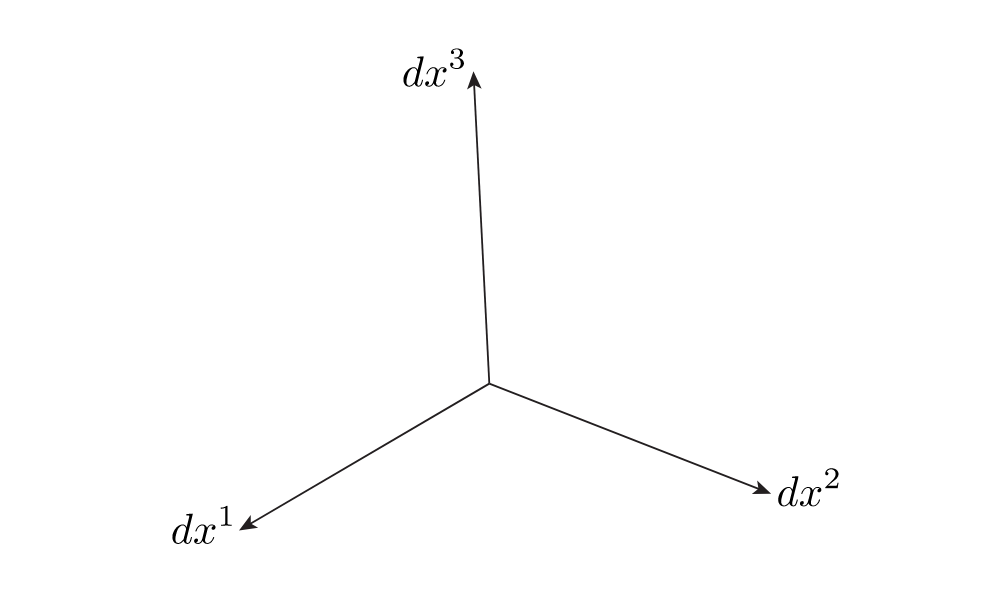
\includegraphics[width=.8\columnwidth]{1forms.png}
%\end{figure}
%\vfill
%\end{frame}
%
%\begin{frame}{2-Forms}
%\begin{figure}[H]
%    \centering
%	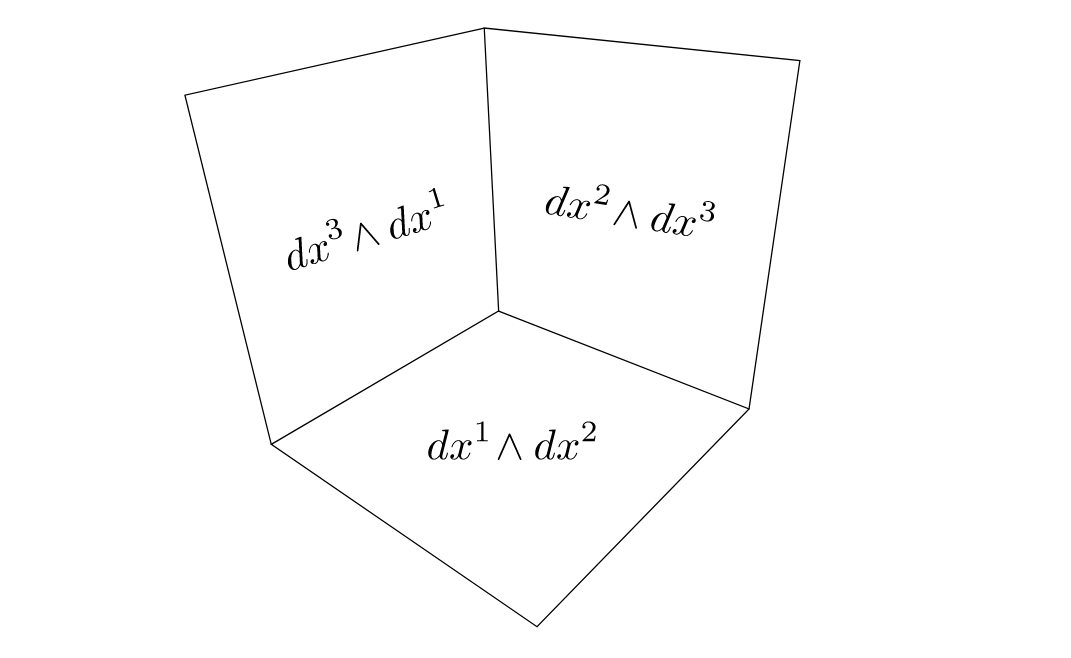
\includegraphics[width=.8\columnwidth]{2forms.png}
%\end{figure}
%\vfill
%\end{frame}
%
%\begin{frame}{3-Forms}
%\vfill
%\begin{figure}[H]
%    \centering
%	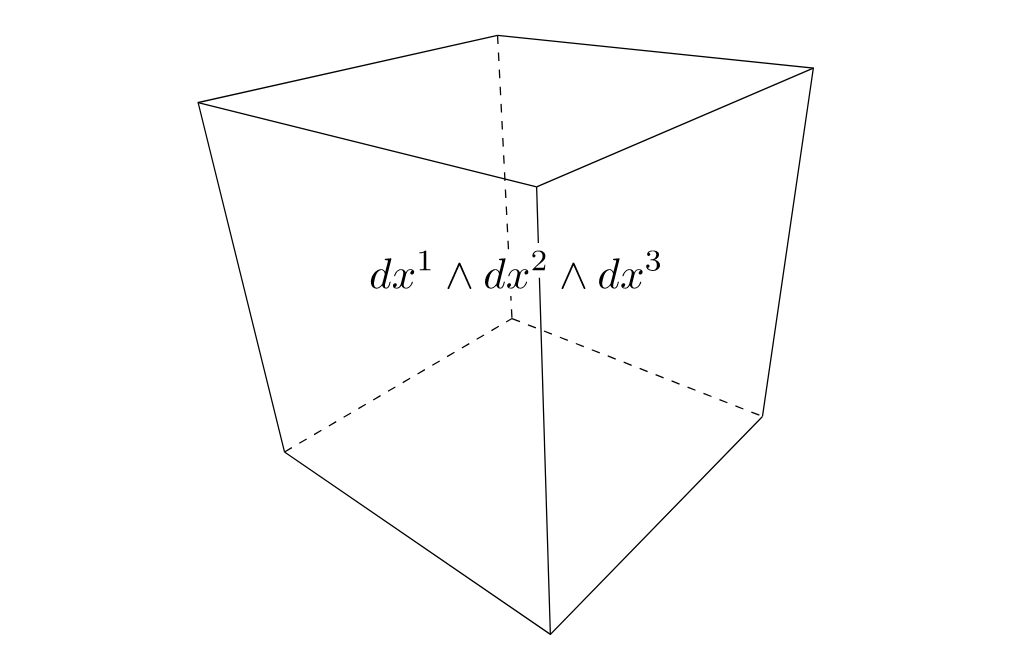
\includegraphics[width=.8\columnwidth]{3forms.png}
%\end{figure}
%\vfill
%\end{frame}
%
%
%
%
%\begin{frame}{Partial Differential Equations}
%    \vfill
%    \pause
%    \begin{itemize} 
%    \item \boldgreen{$k$-Form Inner Product}: $\displaystyle{\langle\alpha,\beta\rangle = \int_\Omega \alpha \wedge \star \beta}$.
%    \pause
%    
%        \item \boldgreen{Exterior Derivative}: Derivative operator $d$ defined on $k$-forms.  
%        
%        \pause 
%        \item \boldgreen{Codifferential}: Formal adjoint to $d$ written as $\delta$.
%        
%        \pause
%        \item \boldgreen{Dirac Operator}: $D=d+\delta$.
%        
%        \pause
%        \item \boldgreen{Laplace-Beltrami Operator}: $\Delta = d\delta +\delta d=D^2$ and in coordinates
%        \[
%        \Delta f = \frac{1}{\sqrt{|g|}} \sum_{j=1}^n \sum_{k=1}^n \frac{\partial}{\partial x^i} \sqrt{|g|} g^{ij} \frac{\partial}{\partial x^j} f 
%        \]
%    \end{itemize}
%\end{frame}
%
%\subsection{Raphrasing EIT Problem in a Geometrical Language}
%

%
%\subsection{Expected and Current Results}
%
%\begin{frame}{Formal Variable Count}
%    \pause $f \mapsto \Lambda(f)$ approximated by
%    \[
%    \Lambda(f)_j = \sum_{k=1}^m \lambda_{jk} f_k.
%    \]
%    
%    \pause In the smooth setting,
%    \[
%    \Lambda(f) = \int_{\partial \Omega} \lambda(x,y) f(y)dS(y).
%    \]
%    
%    \pause So, $g$ is a function of $n$ variables that needs to be determined by the kernel $\lambda$ which is $2n-2$ variables.
%\end{frame}
%
%\begin{frame}{Formal Variable Count}
%\vfill
%\begin{itemize}
%    \pause 
%    \item $n=1$ gives us an undetermined system.
%    
%    \pause
%    \item $n=2$ is well determined.
%    
%    \pause
%    \item $n\geq 3$ is overdetermined.
%   \end{itemize}
%\vfill   
%\end{frame}
%
%
%
%
%\section{Boundary Control Method in 2 Dimensions}
%
%\begin{frame}{Theorem}
%    \pause
%    \emph{Two $2$-dimensional compact orientable manifolds with single common boundary are conformally equivalent iff their DN-maps coincide.}\\
%    
%    \vspace*{1cm}
%    Belishev's \emph{The Calder\'on Problem for Two-Dimensional Manifolds by the BC-Method.}
%\end{frame}
%
%
%\begin{frame}{Key Ideas}
%\vfill
%\pause
%    \begin{itemize}
%        \item Surfaces are two dimensional and can be related to $\C$.
%        
%        \pause
%        \item Holomorphic functions have components that are harmonic.
%        
%        \pause
%        \item Hilbert transform converts one harmonic function to another by connecting them via a single holomorphic function.
%        
%        \pause
%        \item Gelfand transform relates an algebra $\algebra$ to the algebra of continuous functions on the spectrum of that algebra, $C(\spec \algebra)$.
%        
%        \pause
%        \item This gives us a way to realize $\Omega$ from functions defined on $\Omega$ that we have access to.
%    \end{itemize}
%\vfill
%\end{frame}
%
%\begin{frame}{Outline of the Proof}
%\vfill
%\pause
%    \begin{itemize}
%        \item From DN map, recover the algebra of holomorphic functions. (Lemma 1)
%        
%        \pause
%        \item Show that this algebra is generic. (Lemma 2)
%        
%        \pause
%        \item Represent the trace algebra with the DN map. (Lemma 3)
%        
%        \pause
%        \item Construct the manifold. (Theorem)
%    \end{itemize}
%\vfill
%\end{frame}
%
%\begin{frame}{Some Notes}
%    \vfill
%    \begin{itemize}
%    \pause
%    \item We have the inclusion of the boundary $\iota \colon \partial \Omega \to \Omega$.
%    
%    \pause
%    \item The pullback $\iota^* \colon T^*\Omega \to T^*\partial \Omega$.
%    
%    \pause
%    \item Define $\Lambda$ by $\iota^*(\star d u)$ for a harmonic $u$.
%    
%    \pause
%    \item $\Lambda$ maps boundary $k$-forms to boundary $n-k-1$ forms.
%    \end{itemize}
%\end{frame}
%
%\begin{frame}{}
%\begin{figure}[H]
%    \centering
%	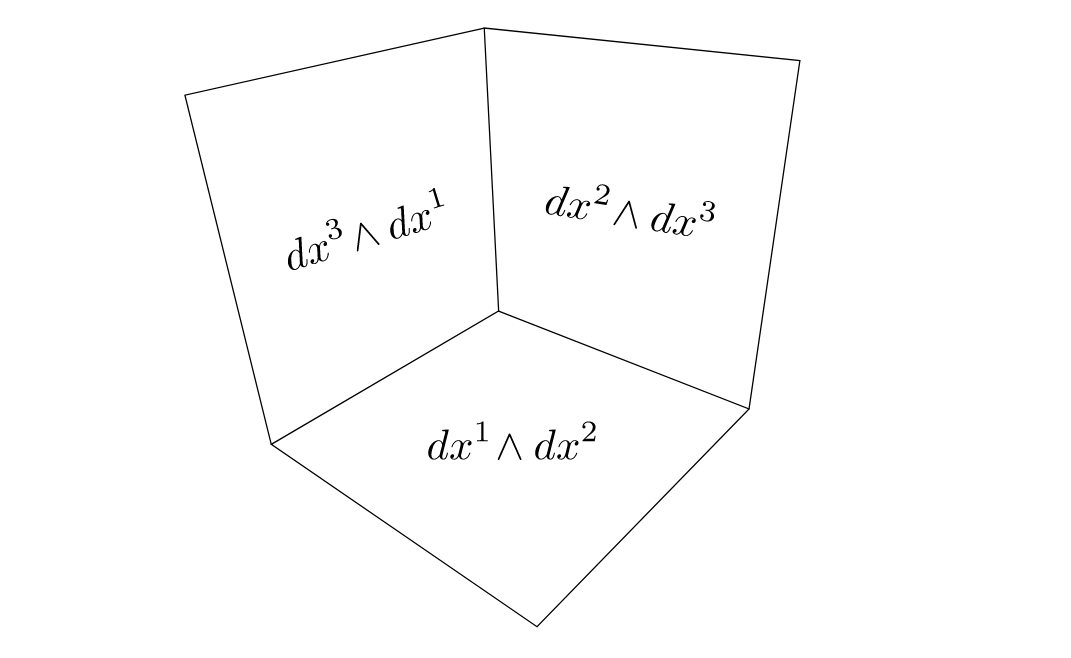
\includegraphics[width=.8\columnwidth]{2forms.png}
%\end{figure}
%\vfill
%\end{frame}
%
%\subsection{Lemma 1}
%
%\begin{frame}{Lemma 1}
%\vfill
%        \begin{itemize}
%            \pause
%            \item A function $u$ satisfying $\Delta u =0$ has a conjugate function $v$ if and only if the trace $\iota^* u$ satisfies
%            \[
%                \left[ \Lambda + d\Lambda^{-1} d\right] \iota^*u = 0.
%            \]
%            
%            \pause
%            \item $\dim\textrm{Ran}\left[ \Lambda + d \Lambda^{-1} d \right] = \beta_1(\Omega).$
%        \end{itemize}
%        \vfill
%\end{frame}
%
%\begin{frame}{Corollary}
%\vfill
%    $\Lambda$ completely determines the topology of $\Omega$.
%\vfill
%\end{frame}
%
%\begin{frame}{Proof}
%\vfill
%\pause
%    \begin{itemize}
%        \item Since $\Omega$ is a single connected component, $\beta_0(\Omega)=1$.
%        \item We have $\beta_1(\Omega)$ from before.
%        \item Since $\Omega$ is a surface with boundary, $\beta_2(\Omega)=0$.
%        \item Since $\Omega$ is two dimensional, $\beta_n(\Omega)=0$ for $n\geq 3$.
%    \end{itemize}
%\vfill
%\end{frame}
%
%\begin{frame}{Conjugate Function Intuition}
%\vfill
%\begin{itemize}
%   \pause
%   \item Suppose we have homorphic complex function $w = u + i v$.  
%   
%   \pause
%   \item Let $u$ be a 0-form and $v$ as a 2-form.
%   
%   \pause
%   \item Then $\frac{\partial}{\partial \overline{z}}$ is given by $D=d+\delta$.
%   
%   \pause
%   \item $Dw=0$ gives us the Cauchy-Riemann equations
%    
%   \item We call $u$ and $v$ conjugate by CREs.    
%\end{itemize}
%\vfill
%\end{frame}
%
%\begin{frame}{Hilbert Transform}
%\vfill
%\begin{itemize}
%    \pause
%    \item We can get $v$ from $u$ via the Hilbert transform.
%    
%    \pause
%    \item Define $\hilbert = d \Lambda^{-1}$.
%\end{itemize}
%\vfill
%\end{frame}
%
%\begin{frame}{Construct the Algebra $\algebra(\Omega)$}
%\vfill
%\begin{itemize}
%    \pause
%    \item By Lemma 1 we can now create the algebra $\algebra(\Omega)\subset C(\Omega)$ from harmonic functions $u$ with conjugates $v$ by
%    \[
%    \algebra(\Omega) \coloneqq \{ w = u+iv\}.
%    \]
%    Algebra since product of two holomorphic functions is holomorphic.
%    
%    \pause
%    \item In isothermal coordinates, each $w\in \algebra(\Omega)$ is holomorphic.
%    
%    \pause
%    \item This gives $\Omega$ a complex structure.
%    
%    \pause
%    \item This is analogous to having the Hodge star on a surface.
%\end{itemize}
%\vfill
%\end{frame}
%
%\subsection{Lemma 2}
%
%
%\begin{frame}{Gelfand Representation}
%\vfill
%    \begin{itemize}
%    \pause
%            \item Let $\functionals$ be the set of multiplicative linear functionals on a commutative Banach algebra $\algebra$.
%            
%        \pause
%        \item The Gelfand transform gives a way of representing an algebra $\algebra$ as a function algebra $\hat{\algebra}$.
%        
%        \pause
%        \item The \boldgreen{Gelfand transform} maps $a\in \algebra$ to a function $\hat{a}$ on $\functionals$ by
%        \[
%        \hat{a}(\delta) \coloneqq \delta(a), \quad \delta \in \functionals.
%        \]
%        
%        \pause
%        \item The \boldgreen{Gelfand topology} is the weakest topology on $\functionals$ in which all $\hat{a}$ are continuous. This makes $\functionals$ compact.
%        
%        \pause
%        \item $\functionals$ with this topology is called the \boldgreen{spectrum} $\spec \algebra$.
%    \end{itemize}
%\vfill
%\end{frame}
%
%\begin{frame}{Generic Algebras}
%\vfill
%    \begin{itemize}
%        \pause
%        \item The Gelfand transform $\hat{\algebra}$ is a subalgebra of $C(\spec \algebra)$ and $a\mapsto \hat{a}$ is an isometric isomorphism.
%        
%%        \pause
%%        \item An isomorphism $t\colon A(X) \to B(Y)$ between two function algebras is \boldgreen{spatial} if there exists a bijection $b \colon X \to Y$ such that $tw=w\circ b^{-1}$.  
%        
%        \pause
%        \item For a function algebra $\algebra \subset C(X)$, take $\epsilon \colon X \to \spec \algebra$ with $\epsilon(x)=\delta_x$.
%        
%        \pause
%        \item A function algebra $\algebra \subset C(X)$ is \boldgreen{generic} if $\epsilon$ is a homeomorphism. 
%        
%        \pause
%        \item A generic algebra is (spatially) isomorphic to its Gelfand transform.
%        
%    \end{itemize}
%\vfill
%\end{frame}
%
%\begin{frame}{Lemma 2}
%\vfill
%\pause
%    The algebra of holomorphic functions $\algebra(\Omega)$ is generic.
%\vfill
%\end{frame}
%
%\begin{frame}{Importance}
%\vfill
%    \begin{itemize}       
%        \pause
%        \item $\hat{\algebra}(\partial \Omega)$ is (spatially) isomorphic to $\algebra(\Omega)$ by taking the Gelfand transform of the trace.
%        
%        \pause
%        \item The lemma shows that $\epsilon \colon \Omega \to \spec \algebra(\Omega)$ is a homeomorphism, so we have determined $\Omega$ up to homeomorphism.
%    \end{itemize}
%\vfill
%\end{frame}
%
%\begin{frame}{What's Left?}
%\vfill
%\pause
%
%    We can only have hope access to the trace algebra $\algebra(\partial \Omega)$. So we need to determine this to reach our goal.
%    \vfill
%\end{frame}

%\begin{frame}{Commutative Banach Algebras (CBA)}
%\vfill
%    \begin{itemize}
%        \pause
%        \item An algebra $\algebra$ is a \boldgreen{commutative Banach Algebra} if 
%        \begin{itemize}
%            \item $\algebra$ is a Banach space.
%            \item $a,b \in \algebra$ satisfy $\|ab\|\leq \|a\|\|b\|$.
%        \end{itemize}
%        
%        \pause
%        \item $\algebra(\Omega) \subset C(\Omega)$.
%        
%        \pause
%        \item $C(\Omega)$ is a CBA and $\algebra(\Omega)$ is a subalgebra.
%        
%        \pause
%        \item $C(\Omega)$ is a \boldgreen{uniform} algebra so $\|a^2\|=\|a\|^2$.
%    \end{itemize}
%\vfill
%\end{frame}
%
%\begin{frame}{Ideals and Functionals}
%\vfill
%    \begin{itemize}
%        \pause
%        \item A subspace $I\neq \algebra$ is an \boldgreen{ideal} if $ja \in I$ for $j\in I$ and $a\in \algebra$.
%        
%        \pause
%        \item An ideal is \boldgreen{maximal} if $\tilde{I}\subset \algebra$ and $I\subset \tilde{I}$ implies $I=\tilde{I}$.
%        
%        \pause 
%        \item A functional $\delta \in \algebra'$ is \boldgreen{multiplicative} if $\delta(ab)=\delta(a)\delta(b)$. 
%        
%        \pause
%        \item Ex: Dirac measure since $\delta_x(ab)=a(x)b(x)$.  
%    \end{itemize}
%\vfill
%\end{frame}

%\begin{frame}{Ideals and Functionals}
%\vfill
%    \begin{itemize}
%        \pause
%        \item Let $\ideals$ be the set of maximal ideals of $\algebra$.
%        
%        \pause
%        \item Let $\functionals$ be the set of multiplicative functions on $\algebra$.
%        
%        \pause
%        \item These sets are in bijection. 
%        
%        \begin{itemize}
%            \item If $\delta \in \functionals$ then $I_\delta \coloneqq \ker \delta \in \ideals$.  
%            \item If $I\in \ideals$ then $\delta_I \colon \algebra \to \algebra / I = \C$ is in $\functionals$.
%        \end{itemize}
%    \end{itemize}
%\vfill
%\end{frame}






%\subsection{Lemma 3}
%
%\begin{frame}{Trace Algebra}
%\vfill
%    \begin{itemize}
%        \pause
%        \item The trace algebra $\algebra (\partial \Omega) \coloneqq \iota^* \algebra(\Omega)$ is isometrically isomorphic to $\algebra(\Omega)$ since
%        \[
%        \|w\|_{\algebra(\Omega)} = \|\iota^* w \|_{\algebra(\partial \Omega)}
%        \]
%        and since a holomorphic function is uniquely determined by its boundary values.
%    \end{itemize}
%\vfill
%\end{frame}
%
%\begin{frame}{Lemma 3}
%\vfill
%    We have the representation
%    \[
%    \algebra(\partial \Omega) = \mathrm{clos}_{C(\partial \Omega)} \{ f +i h\},
%    \]
%    where $h$ is conjugate to $f$ by $\hilbert$.
%\vfill
%\end{frame}
%
%\subsection{Proof of the Main Theorem}
%
%
%\begin{frame}{Construction of the Manifold}
%\vfill
%\pause
%Following these steps yields a manifold $(\Omega, g)$ with the DN map $\Lambda$.
%    \begin{itemize}
%        \pause
%        \item \underline{Step 1:} We know $g|_{\partial \Omega}$ by Lee and Uhlmann, and thus we know $\hilbert$ and $C^\infty(\partial \Omega)$.  This allows us to recover the trace algebra $\algebra(\partial \Omega)$ using the representation in Lemma 3.
%        
%        \pause
%        \item \underline{Step 2:} Then find $\spec \algebra(\partial \Omega)=\Omega$ by Lemma 2.
%        
%        \pause 
%        \item \underline{Step 3:} Next, the Gelfand transform $\hat{\algebra}(\partial \Omega)=\algebra(\Omega)$ by Lemma 2.
%        
%        \pause
%        \item \underline{Step 4:} $\algebra(\Omega)$ gives us the complex structure on $\Omega$ by Lemma 1.
%        
%        \pause
%        \item \underline{Step 5:} Equip $\Omega$ with a metric $g$ conforming to this complex structure.
%    \end{itemize}
%\vfill
%\end{frame}
%
%
%
%
%\section{Generalizing This Method}
%
%\begin{frame}{First Issue}
%\vfill
%\pause
%    \begin{itemize}
%        \item No complex structure in higher dimensions.
%    \end{itemize}
%    \vfill
%\end{frame}
%
%\begin{frame}{Resolution}
%\vfill
%\pause
%    \begin{itemize}
%        \item Use a Clifford algebra/calculus structure to replace $\C$.
%        
%        \pause
%        \item The tools of Clifford analysis allow us to recover a notion of holomorphicity known as \boldgreen{monogenicity}.
%        
%        \pause
%        \item We can recover a similar algebra (Hardy space) of monogenic functions.
%    \end{itemize}
%\vfill    
%\end{frame}
%
%\begin{frame}{Clifford Structure}
%\vfill
%    A Clifford algebra builds upon the exterior algebra of forms.  Given a quadratic space $(V,Q)$, we have
%    \pause
%    \begin{itemize}
%        \item The quotient of the tensor algebra
%        \[
%        \clifford(V,Q) =\quotient{\bigoplus_{j=0}^\infty V^{\otimes j}}{\langle v \otimes v - Q(v)\rangle}.
%        \]
%        
%        \pause
%        \item If $Q=g$ is an inner product, this yields a geometric product on vectors $u,v \in \clifford(V,g)$
%        \[
%        uv = g(u,v) + u\wedge v.
%        \]
%        
%        \pause
%        \item Geometric product can be extended to multivectors.
%    \end{itemize}   
%\vfill
%\end{frame}
%
%\begin{frame}{Familiar Examples}
%\vfill
%\pause
%We have all seen Clifford algebras before.  Indeed, 
%\pause
%\begin{itemize}
%    \item $\C \cong \clifford(\R,-\cdot)$.
%    
%    \pause
%    \item $\C$ also lives inside of $\clifford(\R^2,\cdot)$ as the even subalgebra. That is,
%    \[
%    x+iy \iff 1x + e_1 \wedge e_2 y,
%    \]
%    where $e_1\wedge e_2$ is the bivector (and psuedoscalar).  
%    \pause
%    \item $\mathbb{H}$ lives inside of $\clifford(\R^3,\cdot)$ as the even subalgebra.
%\end{itemize}
%\vfill
%\end{frame} 
%
%\begin{frame}{Clifford Analysis}
%\vfill
%\begin{itemize}
%\pause
%
%    \item We can replace $d+\delta$ with the Dirac operator $D$
%    \[
%    D = \sum_{j=1}^n e_j \frac{\partial}{\partial x^j}.
%    \]
%    
%    \pause
%    \item $D^2 = \Delta$.
%    
%    \pause
%    \item Elements in the kernel of $D$ are monogenic.
%    
%    \pause
%    \item Monogenic objects in even subalgebra have components that are harmonic.
%    
%    \pause
%    \item There are Cauchy integral and Hilbert transform type operators for $D$ in arbitrary dimension.
%    \end{itemize}
%    \vfill
%\end{frame}
%
%\begin{frame}{Second Issue}
%    In dimensions greater than 2, even subalgebra is noncommutative.
%    \begin{itemize}
%        \pause
%        \item The spectral theory for Belishev's solution required a commutative Banach algebra.
%        
%        \pause
%        \item The spectral theory for noncommutative Banach algebras is not as developed.
%        
%        \pause
%        \item There is still work to do here to find some way around this.
%    \end{itemize}
%\end{frame}
%
%\section{Conclusion}
%
%\begin{frame}{Main Story}
%    \begin{itemize}
%        \pause
%        \item Calder\'on proposed a useful and challenging problem for both theorists and practicioners.
%        
%        \pause
%        \item Advances have been made in both areas.
%        
%        \pause
%        \item Ideal results are still not yet obtained.
%    \end{itemize}
%\end{frame}
%
%\begin{frame}{Novel Approach}
%    \begin{itemize}
%        \pause
%        \item Belishev solved the 2D problem using the boundary control method.
%        
%        \pause
%        \item It relies heavily on complex analysis and the spectral theory for commutative Banach algebras.
%        
%        \pause
%        \item These issues remain if we try to naively generalize this approach.
%    \end{itemize}
%\end{frame}
%
%\begin{frame}{New Input}
%    \begin{itemize}
%        \pause
%        \item Clifford algebras and analysis replace the complex structure in arbitrary dimension.
%        
%        \pause
%        \item We can still construct the same algebra of holomorphic functions.
%        
%        \pause
%        \item The relevant algebras are noncommutative for dimensions $\geq$ 3.
%        
%        \pause
%        \item There are possibly other tools at our disposal that may be able to replace the loss of commutivity.
%    \end{itemize}
%\end{frame}
%
%\begin{frame}{}
%    \vfill
%    \centering \huge{Thank you!}
%    \vfill
%\end{frame}


%\section*{Bibliography}
%
%\begin{frame}{References}
%    \begin{itemize}
%        \item \url{http://www.numdam.org/article/SLSEDP_2012-2013____A13_0.pdf}
%        \item Dirichlet to Neumann operator on differential forms
%        \item 2d bc method
%        \item The HIlbert Transform on a smooth closed hypersurface
%    \end{itemize}
%\end{frame}
